\documentclass[11pt,letterpaper]{article}
\usepackage[numbers,sort&compress]{natbib}
\usepackage{graphicx, geometry, amsmath, hyperref, url, booktabs, longtable, array, xcolor, listings, xurl}
\geometry{margin=1in}
\hypersetup{colorlinks=true, linkcolor=black, citecolor=black, urlcolor=black}
\renewcommand{\topfraction}{0.9}
\renewcommand{\bottomfraction}{0.8}
\renewcommand{\textfraction}{0.07}
\renewcommand{\floatpagefraction}{0.75}
\Urlmuskip=0mu plus 1mu

\title{Isothermal Barometric Boiling Points Match a Computed Table to 0.6 K}
\author{}
\date{}

\begin{document}
\maketitle

\begin{abstract}
The boiling point of water falls with altitude, and it is often estimated by combining the barometric formula with the Clausius-Clapeyron equation, which relates vapour pressure to temperature through the enthalpy of vaporisation. We set out to measure how well this estimate predicts measured boiling temperatures at altitude. The headline is a computed agreement, not a measured one. The isothermal barometric model with a constant enthalpy of vaporisation lies within 0.6 K of the Engineering ToolBox table from 0 to 9.1 km, with a mean residual of $+0.50$ K at 6 to 9 km (no interval, because the computation is deterministic) and a maximum absolute residual of 0.59 K. This is a single exploratory estimate on 119 altitudes, against a computed reference. It is consistent with that reference and is not an accuracy result. Two later computations on the same table gave $+0.47$ K at 6 km and above. The scope is bounded by the table itself. Its method is unstated, it tracks an International Standard Atmosphere (ISA) calculation below 5 km, and the method behind it above 5 km is unidentified. No measured boiling-point and station-pressure pair was recoverable, so the measured criteria could not be evaluated. A second result is that the ISA lapse-rate model with constant enthalpy falls to $-1.64$ K at 6 to 9 km, and the choice of atmosphere model accounts for about 2.1 K there.
\end{abstract}

\section{Introduction}\label{sec:intro}

Water boils at 100 $^\circ$C at standard pressure at sea level, and its boiling temperature falls as the surrounding pressure falls. At 3,000 m the drop is several kelvin. That is enough to lengthen cooking times, change steam sterilisation and shift the readings of boiling-point thermometers used to estimate altitude. Estimating the boiling point at a given altitude is therefore routine, and the usual route chains two standard relations: the barometric formula gives pressure from altitude, and the Clausius-Clapeyron equation gives boiling temperature from pressure.

Published tables give boiling points against altitude \cite{EngineeringToolBox}, but their method is seldom stated. A table with no stated method cannot serve as a measurement, and a model cannot be judged accurate without a comparison against measured boiling temperatures. The gap this study addresses is that accuracy test. How well does the simple barometric formula, combined with the Clausius-Clapeyron equation, predict measured boiling temperatures at altitude? The measured sources we could identify did not yield usable pairs above 5 km, so the question stays open on the measurement side.

We therefore make a narrower contribution. We compare four model combinations with one another and with a computed reference table, and we report what that comparison can and cannot support. An isothermal or ISA pressure profile, followed by an inversion to boiling temperature, gives four predictions at each altitude. We define the constant-enthalpy model as the inversion that uses the Clausius-Clapeyron equation with a constant enthalpy of vaporisation, and the inversion that uses the IAPWS industrial formulation for water and steam the IAPWS model. Their differences from the table show which modelling choice matters.

Our contributions are:
\begin{itemize}
  \item A comparison of four model combinations over 0 to 9.1 km. The isothermal model with constant enthalpy has a mean residual of $+0.50$ K against the Engineering ToolBox table at 6 to 9 km, with a maximum absolute residual of 0.59 K. This is a single exploratory estimate, consistent with the computed reference. It is not an accuracy result.
  \item An estimate of the atmosphere effect. Switching from the isothermal to the ISA pressure model moves the constant-enthalpy model prediction by about $-2.1$ K at 6 to 9 km against the same table. That is larger than the effect of the enthalpy approximation.
  \item A documented null result. No measured boiling-point pairs were available above 5 km, so the measured criteria could not be evaluated and this study makes no accuracy claim against measurement.
\end{itemize}

Section~\ref{sec:related} sets out the prior work, Section~\ref{sec:method} the models and the data, and Section~\ref{sec:results} reports the comparison. Sections~\ref{sec:discussion} and~\ref{sec:limitations} state what the evidence does not reach.

Figure~\ref{fig:overview} gives an overview of the chain from altitude to residual on one worked altitude, and Figure~\ref{fig:headline} shows the band residuals behind the headline.

\begin{figure}[!htbp]
  \centering
  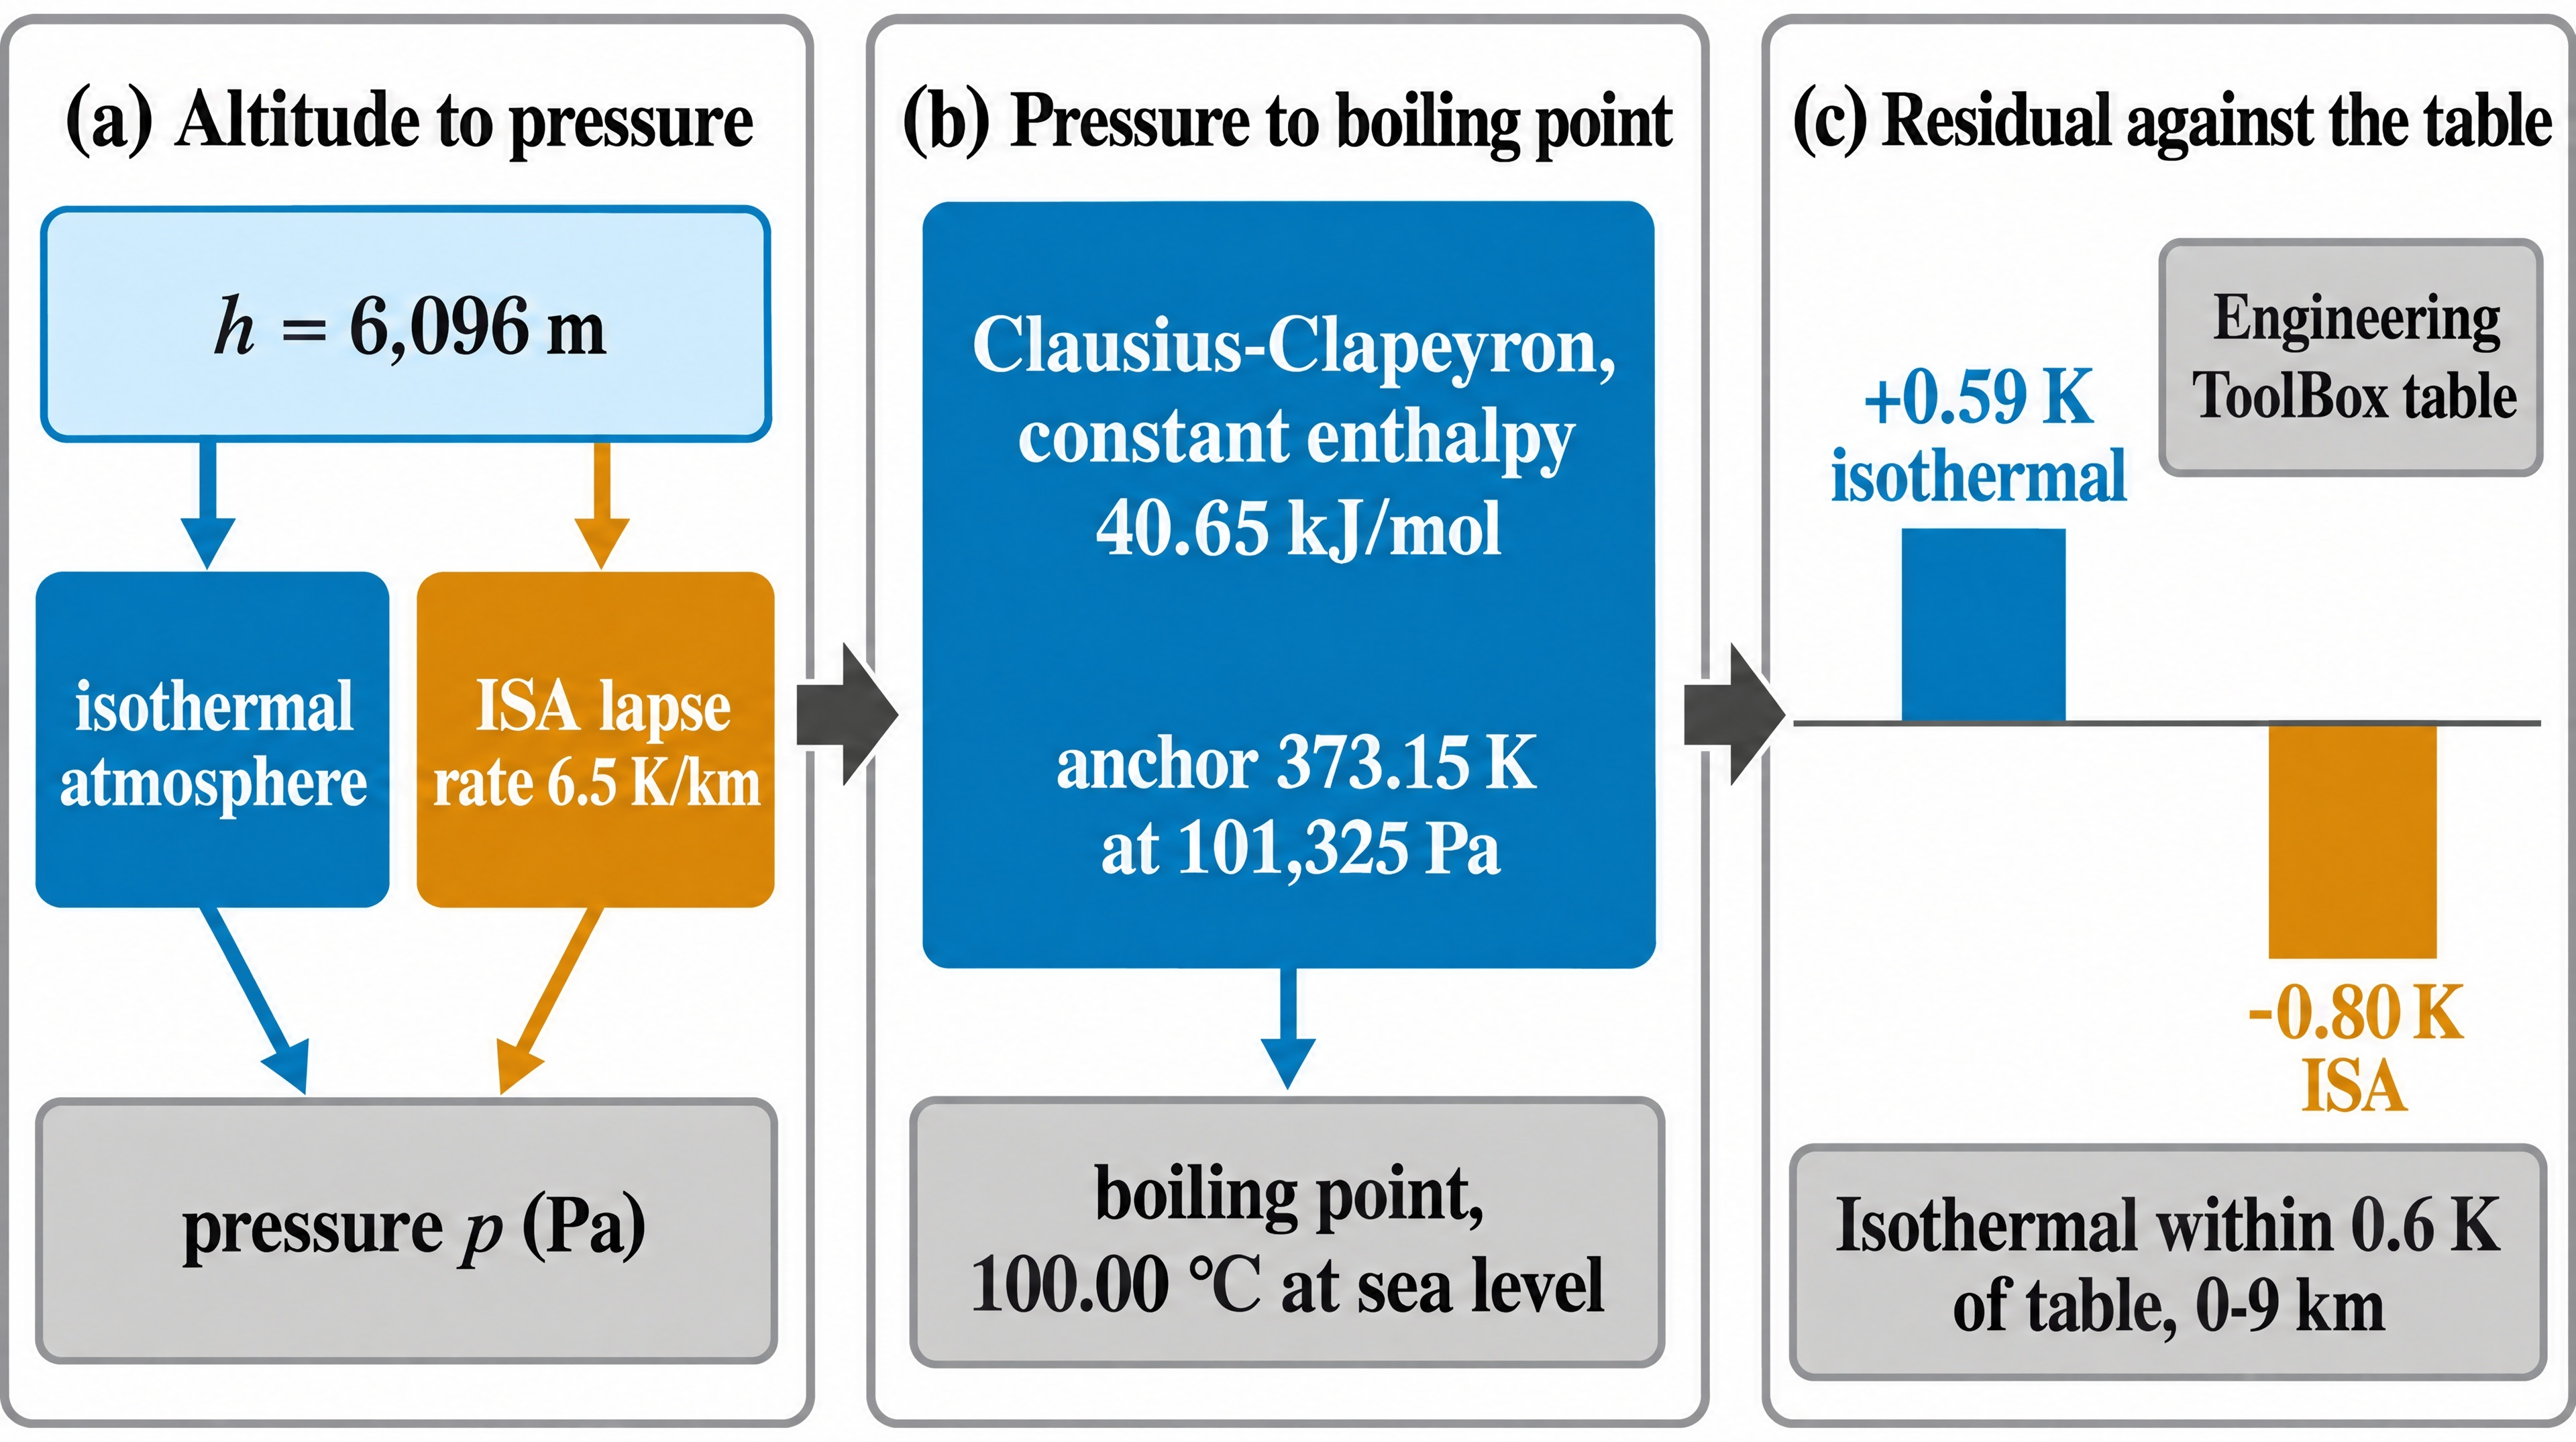
\includegraphics[width=\linewidth,height=0.45\textheight,keepaspectratio]{figures/fig1_v0.jpg}
  \caption{The estimate chains an atmosphere model to a boiling-point model, then compares the result with the Engineering ToolBox table at 6,096 m. Blue marks the isothermal model, orange the ISA model and grey the table; the constant-enthalpy boiling-point step is also drawn blue. Residuals are computed against the table, not measured boiling points.}
  \label{fig:overview}
\end{figure}

\begin{figure}[!htbp]
  \centering
  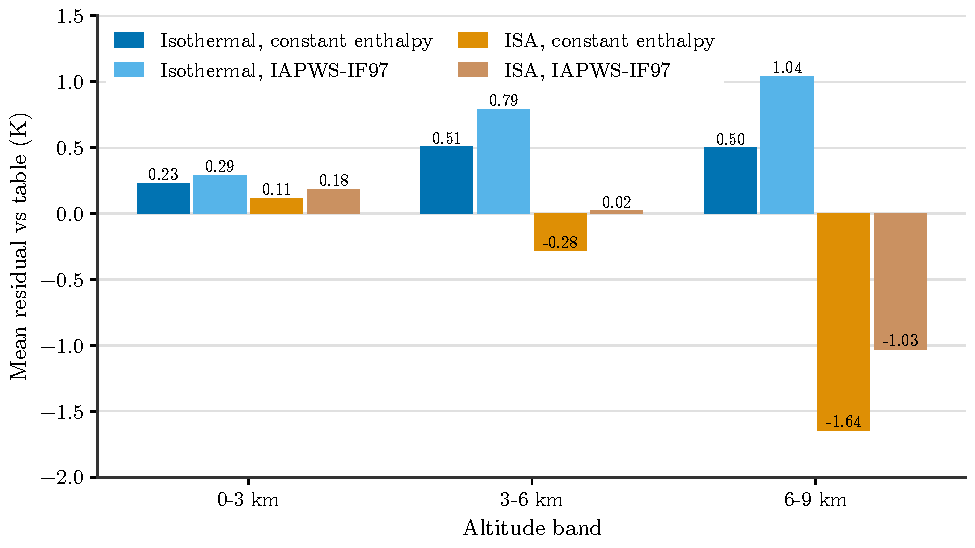
\includegraphics[width=\linewidth,height=0.45\textheight,keepaspectratio]{figures/fig2_v0.pdf}
  \caption{Mean residual in each altitude band (model minus the Engineering ToolBox table) for four model combinations across 119 altitudes from 0 to 9,144 m. Bars show each band's mean without intervals. Isothermal constant enthalpy stays within +0.51 K in every band, while ISA constant enthalpy falls to $-1.64$ K at 6 to 9 km.}
  \label{fig:headline}
\end{figure}

\section{Related Work}\label{sec:related}

\textbf{Atmosphere models.} The isothermal atmosphere gives an exponential pressure profile with a scale height $RT/(Mg)$ \cite{ICAO1993}. The International Standard Atmosphere adds a troposphere with a fixed lapse rate of 6.5 K per km up to 11 km \cite{ICAO1993}. Both are standard and both are widely used. They differ most above 6 km, where the lapse-rate model's cooling accumulates. This study carries both models through to boiling temperature and measures how far their predictions separate, using the same boiling-point inversion for each.

\textbf{Thermodynamics of water and the boiling curve.} The IAPWS formulations give the reference properties of water and steam, including the saturation curve that maps temperature to vapour pressure \cite{Wagner2002,IAPWS1997}. A treatment based on the Clausius-Clapeyron equation with a constant enthalpy of vaporisation is a common shortcut to that curve. This study differs by quantifying how much of the residual due to the atmosphere model the shortcut contributes, with the IAPWS model as its comparator.

\textbf{Boiling-point tables and measurements.} Osborne, Stimson and Ginnings measured the heat of vaporisation and related data for water over 0 to 100 $^\circ$C \cite{Osborne1939}. This study planned to use that work as a measured benchmark, but its values could not be transcribed here. The Engineering ToolBox table gives boiling points from sea level to 9,144 m without a stated method \cite{EngineeringToolBox}. This study treats that table as a computed reference rather than a measurement, and it reports how far the table departs from a ISA calculation.

\section{Method}\label{sec:method}

\subsection{Models}

Pressure comes from one of two atmosphere models. The isothermal model uses a single scale height for the whole range. The ISA model uses the standard troposphere with a 6.5 K per km lapse rate \cite{ICAO1993}. Pressure is then converted to boiling temperature by one of two thermodynamic models. The constant-enthalpy model applies the Clausius-Clapeyron equation with a constant enthalpy of vaporisation of 40.65 kJ/mol, anchored at 373.15 K and a pressure at sea level of 101,325 Pa. The IAPWS model inverts the IAPWS saturation curve \cite{IAPWS1997} by a numerical root-finding inversion, which solves for the boiling temperature at a given pressure. The four combinations are therefore: isothermal with constant enthalpy, isothermal with the IAPWS model, ISA with constant enthalpy, and ISA with the IAPWS model.

\subsection{Reference data}\label{sec:refdata}

The primary reference is the Engineering ToolBox table \cite{EngineeringToolBox}, whose method is not stated. The computed reference is the IAPWS saturation curve evaluated at ISA pressures for the same altitudes, which we call the ISA saturation reference. The reference set holds 250 rows, 125 from each source, and no measured rows. The first computation used 119 altitudes from 0 to 9,144 m. The two later computations used 125 altitudes from $-305$ m to 9,144 m.

\subsection{Metrics}

The residual is model minus table, in kelvin, at each altitude. Within each altitude band (0 to 3 km, 3 to 6 km, and 6 km and above), we report the bias (the mean signed residual), the mean absolute error and the maximum absolute error. The 6 km and above band includes 9,144 m.

\subsection{Measured data and protocol}

The study planned to compare the models with measured boiling temperatures and station pressures from Osborne et al. \cite{Osborne1939} and a CRC Handbook table. Neither source yielded a transcribable table, and the NIST RP1229 document could not be parsed. Zero measured pairs were retained, and no row was padded from a computed table. The measured criteria of the study therefore could not be evaluated. Keene (1995) was not located.

\subsection{Sensitivity and checks}\label{sec:sensitivity}

Moving the anchor from 373.124 K to 373.15 K shifts the constant-enthalpy model predictions by about $+0.02$ K. Changing the enthalpy of vaporisation by $\pm 500$ J/mol changes them by about 0.17 K. The IAPWS model returns 373.124 K at 101,325 Pa, and an independent recalculation reproduced the band statistics.

\section{Results}\label{sec:results}

\subsection{Headline comparison}\label{sec:headline}

The headline is the residual of the isothermal model with constant enthalpy against the Engineering ToolBox table. At 6 to 9 km its mean residual is $+0.50$ K, and its maximum absolute residual across the 119 altitudes is 0.59 K. This is a single exploratory estimate, consistent with the computed reference, with no test fixed in advance or held out from development behind it. The measured criteria could not be evaluated, so this is not an accuracy result. No interval is reported, because the computation is deterministic.

Table~\ref{tab:bands} gives the residuals in each altitude band for every combination against the same table. The isothermal model with constant enthalpy stays closest to the table across the range. Its bias is $+0.23$ K at 0 to 3 km, $+0.51$ K at 3 to 6 km and $+0.50$ K at 6 to 9 km. Figure~\ref{fig:headline} plots the same band means.

\begin{table}[!htbp]
  \centering
  \caption{Mean residual against the Engineering ToolBox table (K), 119 altitudes from 0 to 9,144 m. Residuals are deterministic, so no variance applies.}
  \label{tab:bands}
  \begin{tabular}{>{\raggedright\arraybackslash}p{0.28\linewidth}>{\centering\arraybackslash}p{0.14\linewidth}>{\centering\arraybackslash}p{0.14\linewidth}>{\centering\arraybackslash}p{0.14\linewidth}>{\centering\arraybackslash}p{0.14\linewidth}}
    \toprule
    Combination & Bias 0--3 km & Bias 3--6 km & Bias 6--9 km & Max absolute residual \\
    \midrule
    Isothermal, constant enthalpy & 0.23 & 0.51 & 0.50 & 0.59 \\
    Isothermal, IAPWS model & 0.29 & 0.79 & 1.04 & 1.12 \\
    ISA, constant enthalpy & 0.11 & $-0.28$ & $-1.64$ & 2.60 \\
    ISA, IAPWS model & 0.18 & 0.02 & $-1.03$ & 1.81 \\
    \bottomrule
  \end{tabular}
\end{table}

\subsection{Replication across computations}\label{sec:replication}

Two later computations recomputed the same comparison on the 125-altitude set. Table~\ref{tab:replication} sets the results side by side. The isothermal model with constant enthalpy gives $+0.47$ K at 6 km and above in both later computations, and its largest residual on that set is 0.57 K. The ISA model with constant enthalpy gives $-1.64$ K on the first grid and $-1.72$ K on the second. All three computations use the same Engineering ToolBox table, so their agreement shows that the arithmetic is reproducible. It does not show that the table is accurate.

\begin{table}[!htbp]
  \centering
  \caption{Mean residual against the table at 6 km and above (K). The first column gives the 6 to 9 km band.}
  \label{tab:replication}
  \begin{tabular}{>{\raggedright\arraybackslash}p{0.28\linewidth}>{\centering\arraybackslash}p{0.17\linewidth}>{\centering\arraybackslash}p{0.17\linewidth}>{\centering\arraybackslash}p{0.17\linewidth}}
    \toprule
    Combination & First computation (119 altitudes) & Second computation (125 altitudes) & Third computation (125 altitudes) \\
    \midrule
    Isothermal, constant enthalpy & $+0.50$ & $+0.47$ & $+0.47$ \\
    ISA, constant enthalpy & $-1.64$ & $-1.72$ & $-1.03$ to $-1.72$ (ISA variants) \\
    \bottomrule
  \end{tabular}
\end{table}

\subsection{Atmosphere and enthalpy effects}\label{sec:effects}

Figure~\ref{fig:atmosphere} shows the residual against altitude for the four combinations. The isothermal and ISA curves separate from about 3 km upward. Over 6 to 9 km the atmosphere effect, meaning ISA minus isothermal with both using constant enthalpy, averages about $-2.1$ K. Replacing the constant enthalpy with the IAPWS model in the ISA model removes 37 to 40 percent of its 6 to 9 km bias, and it increases the isothermal model's bias. The anchor shift is a minor term.

\begin{figure}[!htbp]
  \centering
  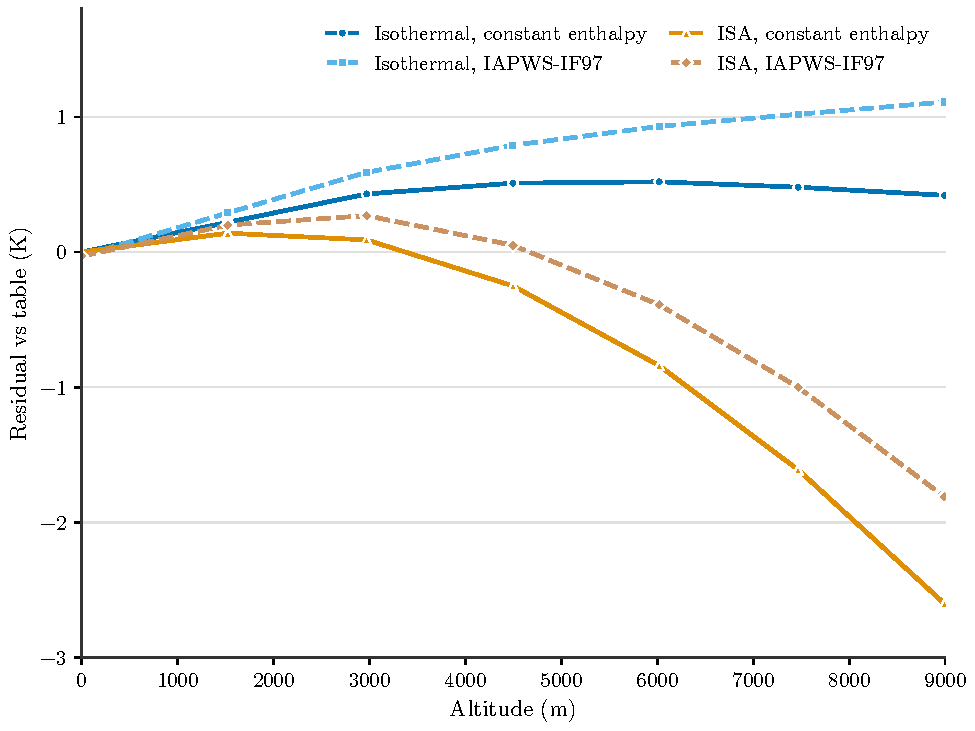
\includegraphics[width=\linewidth,height=0.45\textheight,keepaspectratio]{figures/fig3_v0.pdf}
  \caption{Residual of four boiling-point models against the Engineering ToolBox table at seven altitudes. Above about 4.5 km the ISA curves (orange) fall steeply, reaching $-2.6$ K and $-1.8$ K at 9 km, while the isothermal curves (blue) stay positive. Solid lines use constant enthalpy; dashed lines use the IAPWS model. Computed against the table, not measurements; no error bars.}
  \label{fig:atmosphere}
\end{figure}

\subsection{Dataset check}\label{sec:datacheck}

Across 125 paired altitudes, the Engineering ToolBox table differs from the ISA saturation reference by $-0.31$ K to $+1.94$ K, with a median of $+0.02$ K. Below 5 km the table lies within $-0.31$ K to $+0.11$ K of the ISA saturation reference. The table therefore tracks a ISA calculation closely at low altitude, and it is most likely computed rather than measured. Agreement with the table is agreement with a computed reference.

\subsection{Measured comparison}\label{sec:measured}

The measured comparison has no data. Every band holds zero measured rows. This is a null outcome. The accuracy of the barometric model against measured boiling temperatures at altitude is untested here.

\section{Discussion}\label{sec:discussion}

The headline says that the simplest combination, an isothermal pressure profile with a constant enthalpy of vaporisation, reproduces the Engineering ToolBox table to within about half a kelvin up to 9.1 km. That is a single exploratory estimate, consistent with the computed reference. It answers the question only as far as the computed evidence reaches, and it says nothing about measured boiling points. The table's method is unstated, and it tracks a ISA calculation. Agreement with it therefore checks the simple model against a computed curve, and a computed curve is itself a model.

The more transferable result concerns which choice matters. The atmosphere model changes the predicted boiling temperature by about 2.1 K at 6 to 9 km. The enthalpy approximation changes it by roughly 0.5 to 0.6 K there, and by less than 0.1 K below 3 km (Table~\ref{tab:bands}). Evaluations of boiling temperature at altitude should therefore report the atmosphere model used. A measured test above 6 km should first discriminate the two atmosphere models, because that is where they diverge.

Three design consequences follow for a measured test. First, it needs station pressure recorded with each boiling temperature, because an altitude alone leaves the barometric formula untested. Second, it needs pairs above 6 km, the band where the models separate. Third, it needs its reference thermodynamic model fixed in advance, because the constant-enthalpy and IAPWS model predictions differ by about 0.5 K above 6 km.

\section{Limitations}\label{sec:limitations}

\begin{itemize}
  \item \textbf{No measured comparison.} Zero measured boiling-point and station-pressure pairs were retained, and no measured band reached the minimum of three samples needed for a statistic. The measured criteria could not be evaluated, and nothing here tests accuracy against measurement.
  \item \textbf{Unstated reference method.} The Engineering ToolBox table's method is unknown. Its method above 5 km is unidentified, since it agrees with none of the four variants there. Its values were transcribed from a summary of the page and were not checked against the source page in this study.
  \item \textbf{Shared reference.} Both reference series rest on the same IAPWS saturation curve. The effective enthalpy fitted to that curve is therefore not independent of the reference.
  \item \textbf{Standard atmosphere only.} The ISA residuals describe a standard atmosphere. A real station departs from it with weather and local conditions.
  \item \textbf{No uncertainty estimates.} The computations are deterministic and give no sampling variance or interval. The two later computations use the same table, so their agreement confirms arithmetic, not the table.
  \item \textbf{Gaps in the search.} Keene (1995) was not located. An ACS article on boiling at altitude (DOI 10.1021/ed067p45) could not be retrieved, so its content is unverified. The IAPWS-95 saturation table in NIST NISTIR 5078 could not be parsed, so that reference check is incomplete.
\end{itemize}

\section{Conclusion}\label{sec:conclusion}

The isothermal barometric model with a constant enthalpy of vaporisation lies within 0.6 K of the Engineering ToolBox table up to 9.1 km. This is a single exploratory estimate, consistent with the computed reference and not an accuracy result. The question the study set out to answer, how well the formula predicts measured boiling points at altitude, remains open. Above 6 km the atmosphere model decides most of the disagreement, with about 2.1 K between the isothermal and ISA models. The next step is a measured comparison: boiling temperatures paired with station pressure above 6 km, with each atmosphere and thermodynamic model stated in advance.

\section*{Code availability}

Code, prompts, raw outputs and the scripts that recompute each number are in the paper's code repository~\href{https://github.com/ai-inventor-papers/ai-invention-fde7b3-simple-barometric-model-vs-boiling-point/tree/main}{[code]}, and Appendix~\ref{app:code} links each result to the folder that produced it.

\bibliographystyle{plainnat}
\bibliography{references}

\clearpage
\appendix

\section{Computation details}\label{app:details}

All computations are deterministic and run in Python. Pressure at sea level is 101,325 Pa. The constant-enthalpy model uses 40.65 kJ/mol with an anchor at 373.15 K. The ISA model uses a 6.5 K per km troposphere lapse rate \cite{ICAO1993}. Bands are 0 to 3 km, 3 to 6 km and 6 km and above. Residuals are model minus table, in kelvin. The 119-altitude grid runs from 0 to 9,144 m, and the 125-altitude set runs from $-305$ m to 9,144 m. Rows below sea level are reported separately as informational. The table's rows came from the Engineering ToolBox page \cite{EngineeringToolBox}, and their transcription is the main unverified input.

\section{Code for each result}\label{app:code}

Each row links the code folder, in the code repository, of the experiment behind a result.

\begin{longtable}{p{0.22\linewidth} p{0.40\linewidth} p{0.30\linewidth}}
  \toprule
  Section & Result & Code folder \\
  \midrule
  \endhead
  Abstract & Headline residual, isothermal with constant enthalpy (Table~\ref{tab:bands}) & \href{https://github.com/ai-inventor-papers/ai-invention-fde7b3-simple-barometric-model-vs-boiling-point/tree/main/round-1/experiment-1}{\texttt{round-1/experiment-1}} \\
  Abstract & Two later computations at 6 km and above (Table~\ref{tab:replication}) & \href{https://github.com/ai-inventor-papers/ai-invention-fde7b3-simple-barometric-model-vs-boiling-point/tree/main/round-2/experiment-2}{\texttt{round-2/experiment-2}}, \href{https://github.com/ai-inventor-papers/ai-invention-fde7b3-simple-barometric-model-vs-boiling-point/tree/main/round-2/experiment-4}{\texttt{round-2/experiment-4}} \\
  \S\ref{sec:refdata} & Reference set and altitude grids (Section~\ref{sec:refdata}) & \href{https://github.com/ai-inventor-papers/ai-invention-fde7b3-simple-barometric-model-vs-boiling-point/tree/main/round-1/dataset-1}{\texttt{round-1/dataset-1}} \\
  \S\ref{sec:headline} & Headline comparison (Table~\ref{tab:bands}, Figure~\ref{fig:headline}) & \href{https://github.com/ai-inventor-papers/ai-invention-fde7b3-simple-barometric-model-vs-boiling-point/tree/main/round-1/experiment-1}{\texttt{round-1/experiment-1}} \\
  \S\ref{sec:replication} & Replication across computations (Table~\ref{tab:replication}) & \href{https://github.com/ai-inventor-papers/ai-invention-fde7b3-simple-barometric-model-vs-boiling-point/tree/main/round-2/experiment-2}{\texttt{round-2/experiment-2}}, \href{https://github.com/ai-inventor-papers/ai-invention-fde7b3-simple-barometric-model-vs-boiling-point/tree/main/round-2/experiment-4}{\texttt{round-2/experiment-4}} \\
  \S\ref{sec:effects} & Atmosphere and enthalpy effects (Figure~\ref{fig:atmosphere}) & \href{https://github.com/ai-inventor-papers/ai-invention-fde7b3-simple-barometric-model-vs-boiling-point/tree/main/round-1/experiment-1}{\texttt{round-1/experiment-1}} \\
  \S\ref{sec:datacheck} & Dataset check against the ISA saturation reference & \href{https://github.com/ai-inventor-papers/ai-invention-fde7b3-simple-barometric-model-vs-boiling-point/tree/main/round-1/dataset-1}{\texttt{round-1/dataset-1}} \\
  \S\ref{sec:measured} & Measured comparison (null outcome) & \href{https://github.com/ai-inventor-papers/ai-invention-fde7b3-simple-barometric-model-vs-boiling-point/tree/main/round-1/research-1}{\texttt{round-1/research-1}} \\
  \S\ref{sec:sensitivity} & Sensitivity checks (Section~\ref{sec:sensitivity}) & \href{https://github.com/ai-inventor-papers/ai-invention-fde7b3-simple-barometric-model-vs-boiling-point/tree/main/round-2/experiment-3}{\texttt{round-2/experiment-3}} \\
  \S\ref{sec:limitations} & Engineering ToolBox transcription (Section~\ref{sec:limitations}) & \href{https://github.com/ai-inventor-papers/ai-invention-fde7b3-simple-barometric-model-vs-boiling-point/tree/main/round-1/research-1}{\texttt{round-1/research-1}} \\
  \bottomrule
\end{longtable}

\end{document}
